\subsection{Proprietà meccaniche}

\epigraph{Nelle zone di estinzione (\textcolor{red}{gli spigoli ad esemio (?)}) come si hanno condizioni triassiali in ogni caso a meno di rotazioni è sempre possibile trovare una forma diagonale del tensore.}{\textit{Leonardo Sabattini}, I edizione}

\begin{itemize}
    \item \textbf{\textit{Durezza}} capacità di un materiale di essere penetrato da un altro.
    \item \textbf{\textit{Rigidezza}} capacità di un materiale di opporsi ad una deformazione (modulo elastico).
    \item \textbf{\textit{Resistenza}} tensione sopportata prima di un cedimento; ce ne sono di vario tipi:
    \begin{enumerate}
        \item \textbf{\textit{ultimate strength} o \textit{carico di rottura}} si riferisce al valore della tensione massima che il campione riesce a sopportare.
         \item \textbf{\textit{yield strength} o \textit{snervamento}} si riferisce al valore della tensione massima prima che il campione si deformi irreversibilmente.
    \end{enumerate}
    \item \textbf{\textit{Resilienza}} energia assorbita prima della rottura.
    \item \textbf{\textit{Tenacità}} energia assorbita prima del punto di snervamento.
\end{itemize}
Quasi tutte queste proprietà possono essere misurate con la prova di trazione mostrata in Fig \ref{fig:prova-trazione}. In questa prova un provino (regolamentato) viene sottoposto a strain rate costante (regolamentata anch'essa).
\begin{figure}[h]
    \centering
    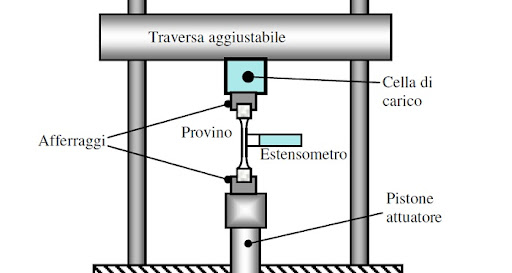
\includegraphics[width=10cm]{Proprietà_meccaniche/prova_trazione.jpg}
    \caption{Set up della prova di trazione}
    \label{fig:prova-trazione}
\end{figure}
La forma del provino è studiata in modo da ottimizzare il processo, la forma ad "osso di cane" permette di evitare la rottura in punti più sensibili come gli spigoli e favorire la rottura nella parte centrale dove il materiale è più omogeneo (il campo di forze non è omogeneo, al di fuori della zona centrale il bilanciamento delle forze non è più semplice).
Il risultato della prova di trazione dipende ovviamente dal materiale e dalle sue caratteristiche. In generale ciò che si misura è lo Stress (Forza/Area) in funzione dello Strain (Allungamento/Lunghezza del provino). Bisogna fare alcuni accorgimenti sulle definizioni che vengono utilizzate, in quanto né la sezione né la lunghezza del campione sono uguali durante il procedere della prova; se si considerano i valori uguali al valore iniziale allora si parla di \textbf{\textit{Engineering Stress e Engineering Strain}}, quando si fa riferimento ai valori istantanei si parla invece di \textbf{\textit{True Stress e True Strain}}. I grafici che si ottengono sono in genere differenti, solo per piccoli spostamenti si ha che queste due diverse quantità tendono allo stesso risultato:
$$\epsilon=\int_i^f\frac{dl}{l}=ln(l_f/l_i)=ln(l_i+\Delta l/l_i)\simeq\frac{\Delta l}{l_i}=\epsilon_{eng}$$
Non c'è da stupirsi di ciò in quanto il campione viene deformato e le lunghezze durante la prova cambiano.
\begin{figure}[h]
    \centering
    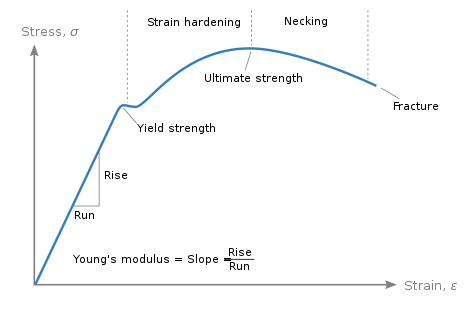
\includegraphics[width=10cm]{Proprietà_meccaniche/stress-strain.png}
    \caption{Stress-Strain curve}
    \label{stress-strain}
\end{figure}
In questi grafici è spesso possibile riconoscere tre zone differenti. Se guardiamo Fig \ref{stress-strain} possiamo vedere l'andamenteo dell'Engineering Stress in funzione dell'Engineering Strain:
\begin{itemize}
    \item In ogni grafico è presente una zona di \textbf{\textit{regime lineare o elastico}} in cui la deformazione è reversibile una volta tolto il carico; l'estensione di questa regione è legata all'intensità delle forze di legame.
    \item Arrivati ad un certo punto chiamato \textbf{\textit{punto di snervamento}} le deformazioni non sono più reversibili e si entra nel cosiddetto \textbf{\textit{regime plastico}}. A volte non è facile individuare questo punto, dunque si definisce per convenzione come punto di snervamento come il punto in cui permane una deformazione del 0.2\% del campione, per ritornare alla condizione iniziale occorre applicare una compressione il cui valore viene definita \textit{tensione residua}. In questo, una volta tolto il carico si ha che il campione non torna più allo stato iniziale ma vi rimane uno stress residuo.
    Non tutti i  materiali presentano questo regime: i materiali fragili si spezzano rimanendo in regime lineare. Il tipo  di rottura può essere duttile o fragile, a seconda della forma con cui si spezza il provino.
    \item Il grafico presenta un massimo detto \textbf{\textit{carico di rottura}}. Raggiunto questo punto si ha una deformazione su tutto il provino si inizia ad assistere al fenomeno di \textbf{\textit{strizione}} ed è considerato \textbf{\textit{failure}} ciò il materiale al di sopra di questo punto non può più essere impiegato. 
    \item Il punto in cui si ha la rottura del campione è detto \textbf{\textit{punto di rottura}}, il fatto che sia a valori più bassi è solo perché stiamo considerando le quantità ingegneristiche, se usassimo i valori reali avremmo una curva monotona crescente in quanto le dimensioni prese in considerazione diminuiscono nel corso della prova.
\end{itemize}
All'interno del regime lineare vale una legge del tipo:
\begin{equation}
    \sigma_{zz}=E\epsilon_{zz}
\end{equation}
$E$ è il modulo di Young ed è anche chiamata rigidezza, viene misurata in [kPa], [MPa] o [GPa]. Il modulo di Young in generale e diverso in base alla direzione ed al punto in cui si osserva, per materiali omogenei e isotropi possiamo ritenerlo costante. Se fossimo nel regime plastico potremmo definire un modulo di Young come: $\frac{d\sigma_{zz}}{d\epsilon_{zz}}$. 
Nel regime lineare, lo strain lungo z è collegato allo strain nelle altre direzioni:
\begin{equation}
    \nu=\frac{\sigma_{yy}}{\sigma_{zz}}=\frac{\sigma_{xx}}{\sigma_{zz}}
\end{equation}
$\nu$ viene chiamato modulo di Poisson è corrisponde alla contrazione della lunghezza trasversale rispetto allo strain; i valori di solito sono compresi tra 0 e 0,5 (per valori di 0,5 si ha la conservazione del volume). Valori inferiori allo 0 sono rari, ma non impossibili, e in questo caso significa durante la deformazione comporta un aumento del volume.
Vediamo ora alcune differenze tra le grandezze reali ed ingegneristiche.
Supponiamo di essere nel regime plastico in cui si ha conservazione del volume, cioè $A_0\cdot l_0=A\cdot l$
Si ha che:
$$\sigma_{eng}=\frac{F}{A_0}=\frac{F}{A}\cdot\frac{l_0}{l}=\sigma\cdot\frac{l}{l_0}$$
$$\epsilon=\int_i^f \frac{dl}{l}=ln(\frac{l_f}{l_i}=ln(\epsilon_{eng}+1)$$
Sopra abbiamo assunto che il materiale sia isotropo, ma in generale questa cosa non è vera e dovremmo avere rapporti di Possion diversi in direzioni diverse.
Con la prova di trazione è possibile ottenere moltissime informazioni, ma non è esaustiva per determinare tutte le proprietà meccaniche del provino; come vedremo più avanti esistono altre prove per misurare, ad esempio, la resistenza a compressione, flessione e torsione.
La resilienza è l'energia assorbita durante il processo in regime elastico, e corrisponde all'area sottostante al grafico (ha le dimensioni di un lavoro per unità di volume), mentre l'area sottesa da tutto il grafico viene definita tenacità; per materiali non isotropi entrambe dipendono dalla direzione in cui si effettua la prova.
$\sigma_{max}$ ci dà informazioni sulla resistenza; in generale per sistemi non omogenei e non isotropi può non essere ben definita in quanto dipende dalla direzione e da come viene effettuata la prova. Il modulo di Young ci dice quanto è rigido un materiale mentre $\epsilon_R$ riguarda la duttilità.
\begin{table}[h]
\centering
\begin{tabular}{@{}llcc@{}}
\toprule
\textbf{Materiale} & \textbf{Descrizione} & \textbf{Resistenza ($MPa$)} & \textbf{Modulo di Young ($GPa$)} \\ \midrule
PET  & Plastica termoplastica & 55 - 75 & 2 - 4 \\
Acciaio (AISI 304) & Acciaio inossidabile austenitico & 210 - 550 & 190 - 210 \\
Alluminio (Al 6061) & Lega di alluminio & 240 - 310 & 68 - 70 \\
Rame (Cu) & Metallo non ferroso & 110 - 220 & 110 - 130 \\
Legno (Pino) & Materiale naturale & 40 - 80 & 10 - 15 \\ \bottomrule
\end{tabular}
\caption{Proprietà meccaniche di alcuni materiali}
\label{tab:proprietà_materiali}
\end{table}


\begin{wrapfigure}{l}{0.43\textwidth}[h]
  \centering
  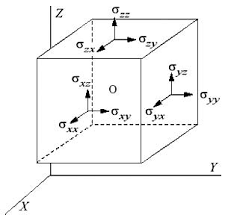
\includegraphics[width=0.26\textwidth]{Proprietà_meccaniche/cubetto.png}
  \caption{cubetto}
  \label{cubetto}
\end{wrapfigure}

Per capire come si comporta macroscopicamente il materiale andremo a vedere come agiscono le tensioni su di un cubetto di dimensioni infinitesime dXdYdZ (Fig \ref{cubetto}): definiamo il tensore degli sforzi: $$\sigma_{ij}$$ dove i indica direzione della normale alla faccia e j invece indica la direzione della forza.
In generale è possibile dimostrare che questo tensore è simmetrico (e quindi anche diagonalizzabile), in caso contrario è possibile dimostrare che esiste un momento torcente non nullo sul nostro cubetto che ne causerebbe la rotazione.
In molti casi pratici si cerca di ricondursi a stress mono- o biassiale, che algebricamente significa ridurre il tensore degli sforzi ad un solo autovalore (condizioni monoassiali) o due autovalori (condizioni biassiali) nonnulli; questo ad esempio è il caso della prova di trazione di materiali omogenei ed isotropi. \textcolor{red}{chiedere a Milazzo come cambia la prova di trazione per materiali inomogenei e anisotropi}. Al tensore degli sforzi è associato un tensore delle deformazioni $\epsilon_{ij}$; in generale la relazione che c'è tra i due è sempre un'applicazione lineare simmetrica ma non è banale (lineare quando ci troviamo nel regime elestico ovviamente). In generale si ha una relazione del tipo:
\begin{equation}
    \sigma_{ij}=E_{ijkl}\epsilon_{kl}
\end{equation}

\subsection{Prova di flessione}

\begin{figure}[h]
    \centering
    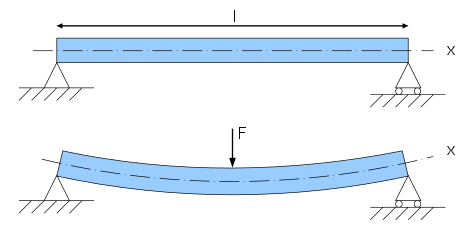
\includegraphics[width=10cm]{Proprietà_meccaniche/prova-flessione.png}
    \caption{Set up della prova di flessione a tre punti, esistono set up in cui sono presenti quattro punti differenti; la dinamica è differente in quanto lo stress subito dai vari punti è differente.}
    \label{fig:prova-flessione}
\end{figure}

La prova di flessione, mostrata in figura \ref{fig:prova-flessione}, consiste nell'applicazione di un provino di forma allungata tre o quattro forze con risultante nulla (si parla rispettivamente di prova a tre o a quattro punti) in punti differenti e su lati opposti del campione. In questo modo non si produce una forza complessiva sul provino, ma viene generato un momento torcente, pertanto alcune zone del materiale sono sottoposte a trazione mentre altre sono sottoposte a compressione. Chiamiamo \textit{fibre} le linee parallele ai due del provino che sono sottoposti a forze; esiste sempre una fibra, detta \textbf{\textit{fibra neutra}}, per cui vale $\sigma_{zz}=0$; tipicamente questa passa per il baricentro del provino, ma vedremo tra poco un'importante eccezione. In generale, soprattutto se il provino non è omogeneo, sapere dove si trova la fibra neutra è importante in quanto i punti più distanti dalla fibra neutra sono quelli in cui si verifica cedimento più facilmente.
Nel caso illustrato in Fig \ref{fig:prova-flessione} vale la legge:
\begin{equation}
    \sigma_x(z)=\frac{M_y}{J_y}z
\end{equation}
Dove $M_y$ è il momento delle forze, $J_y$ è il momento d'inerzia nel piano $xz$ e $z$ è la coordinata nel piano ortogonale alla fibra baricentrica.
Nel regime lineare vale che i contributi si sommano semplicemente, dunque la formula più generale possibile per un corpo sottoposto a flessione su due lati con una trazione (o compressione, più comune soprattutto in ingegneria civile) è:
\begin{equation}
    \sigma_{zz}=\frac{M_x}{J_x}y-\frac{M_y}{J_y}x+F
\end{equation}
dove $F$ è appunto la forza di trazione o compressione. Dal momento che la fibra neutra è quella in cui lo stress è nullo la presenza della forza costante sposta la fibra neutra del baricentro. In generale è possibile osservare che le figure cave come tubi presentano resistenze alle flessioni maggiori in quanto sono quelle che hanno momento d'inerzia maggiore, e questa è una delle ragioni per cui le travi vengono realizzate con forma a doppia T e non sono piene.

\begin{figure}[h]
    \centering
    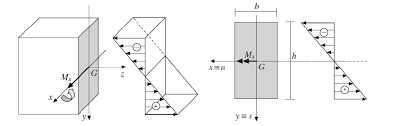
\includegraphics[width=10cm]{Proprietà_meccaniche/fibra neutra.png}
    \caption{Stress percepito da punti in posizioni differenti lungo il campione. La presenza di una forza ha l'azione di traslare il baricentro.}
    \label{fibra-neutra}
\end{figure}

Il test di flessione trova impiego, ad esempio, per la misura delle proprietà dei ceramici. Preparare i campioni dei materiali ceramici per il testi di trazione con le forme adeguate (senza spigoli) non è facile, inoltre anche creare il grip e fissarlo alla macchina senza causare crepe è una cosa non scontata. 
Inoltre si spezzano a valori molto piccoli (0.1\%) e richiede che il campione sia perfettamente allineato senza che esistano stati di flessione in quanto falsano la prova. Il bending test elimina questi problema in quanto la frattura avviene comunque nel lato di trazione.

\subsection{Prova di torsione}

La prova di torsione è tendenzialmente la più complessa da descrivere matematicamente, dato che le equazioni dipendono dalla forma del provino.
Supponiamo di effettuare la prova di torsioni di un cilindro, che è un caso abbastanza comune e semplice. In questo caso la prova di torsione tipica (Fig \ref{prova di torsione}) consiste nel fissare un'estremità mentre all'altra viene applicata un momento torcente.

\begin{figure}[h]
    \centering
    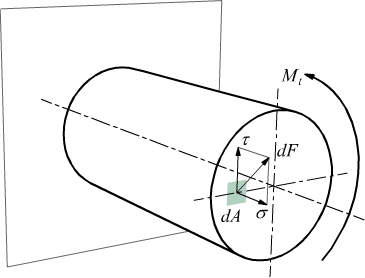
\includegraphics[width=8cm]{Proprietà_meccaniche/provaditorsionemetalli.png}
    \caption{Prova di torsione.}
    \label{prova di torsione}
\end{figure}

In generale la torsione è molto complicata, è possibile farla in maniera semplice solo in alcuni casi ad alta simmetria come la torsione in un cilindro.
La relazione in questo caso è simile alla flessione:
\begin{equation}
    \tau=G\theta
\end{equation}
G che è lo shearing elastic module dipende dalla forma del campione. Nel caso mostrato in figura si ha che:
\begin{equation}
    \tau_{yz}=\frac{M_z}{J_z}r
\end{equation}
Dove $J_z$ è il secondo momento d'inerzia, r è il raggio del cilindro. In ogni caso G non è indipendente da E e da $\nu$ ma nel caso di materiali isotropi ed omogenei vale:
\begin{equation}
    E=2G(1+\nu)
\end{equation}
Per motivi energetici $\nu$ (\textbf{\textit{modulo di Poisson}}) è quasi sempre compreso tra -1 e 1/2.



\subsection{Prove di durezza}
Le prove di durezza consistono nell'osservare la capacità di un materiale nel non essere penetrato da un altro. Esistono diverse prove di durezza:
\begin{itemize}
    \item \textbf{\textit{Brinnel}}: in questa prova si utilizzano delle sfere di materiale duro (WC) con un certo raggio R che vengono pressate sul nostro campione in modo da creare una deformazione permanente (è un test distruttivo ovviamente).
    \begin{equation}
        HB=\frac{F}{\pi 2R P}
    \end{equation}
    F è la forza impressa sulla sfera, P è la profondità con cui penetra il nostro campione; da notare che anche se le dimensioni di HB sono una pressione, questa non ha un vero senso fisico.
    Ovviamente è possibile misurare solo campioni con una durezza minore di WC. La dimensione della sfera è scelta in base la dimensione del campione in quanto misure effettuate con campioni con spessore differente non sono comparabili. Un altra cosa a cui stare attenti è quando si usano materiali troppo morbidi in cui la sfera può completamente entrare, di solito si segue la regola che 0.25<d/D<0.5 dove d è il diametro dell'impronta e D il diametro della sfera. Per confrontare test effettuati con sfere la cui dimensione è diversa di solito si osserva l'angolo, i protocolli più validi sono quelli che lasciano l'angolo uguale in prove differenti.
    
    \item \textbf{\textit{Vickers}}: il test Vickers utilizza invece una punta a forma di prisma (presenta un angolo di 136°) e lavora in microscale andando a misurare la penetrazione (il test può essere considerato non distruttivo).
    \begin{equation}
        HV=\frac{F}{d^2}K
    \end{equation}
    K è un coefficiente numerico (vale 1.854), d è la diagonale del quadrato impresso dal prisma. Questo metodo presenta alcuni problemi, se il materiale è molto morbido la forma impressa potrà essere di difficile interpretazione, inoltre è un metodo molto costoso.
    \item \textbf{\textit{Rockwell}}: in questo test si usa una punta conica con un angolo di 120° in cui sono presenti delle tacche equidistanziate. La durezza è data dal numero di tacche che riescono a penetrare il materiale. Il valore della durezza è dato da:
    \begin{equation}
        HR=100-x
    \end{equation}
    x è il numero di tacche. La presenza di tacche permette calibrazioni
    \end{itemize}
Le relazioni tra test differenti sono difficili, grossolanamente è possibile dire: HR$\simeq$3HB. Nel test Vickers siamo vicini al punto di snervamento (la deformazione è molto piccola), le altre lavorano nel regime plastico.

\subsection{Toughness test}
\begin{figure}[h]
    \centering
    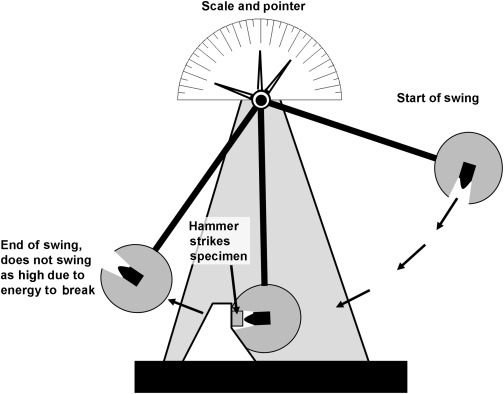
\includegraphics[width=8cm]{Proprietà_meccaniche/toughnesstest.jpg}
    \caption{Toughness test.}
    \label{oughnesstest}
\end{figure}

Il test di tenacità misura la quantità di energia che il materiale riesce ad assorbire prima della rottura. 
In realtà il test di trazione permette di ottenere informazioni sulla tenacità del nostro materiale, spesso però non è sufficiente in quanto le condizioni in cui viene effettuato il test sono fin troppo ideali (situazione di stress uniassiale). In questo test (Fig \ref{oughnesstest}) la forma del campione è diversa in modo da favorire la rottura in un punto specifico. Il principio è rilasciare un peso e misurare l'energia assorbita dal campione nel processo di rottura misurando la differenza di energia potenziale del pendolo.
Ogni test ha una forte dipendenza dalla temperatura, questo è dovuto al fatto che in molti materiali all'aumentare della temperatura si ha un aumento dell'allungamento massimo prima della rottura (il materiale diventa progressivamente più duttile). La cosa molto interessante è che non si ha un aumento lineare con T ma con forma sigmoidale. Il punto d'inversione della derivata seconda è anche detto temperatura di transizione duttile fragile.
Non tutte le strutture presentano questa transizione ed alcune sono più favorite rispetto ad altre come in Fig \ref{duttile-fragile} (\textcolor{red}{chiedere a milazzo perche si ha questo solo per BCC e non FCC}.
\begin{figure}[h]
    \centering
    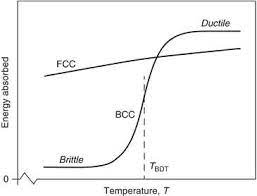
\includegraphics[width=6cm]{Proprietà_meccaniche/duttile-fragile.jpg}
    \caption{Grafico in cui è illustrata una transizione duttile-fragile.}
    \label{duttile-fragile}
\end{figure}